\section{Durchführung}
\label{sec:Durchführung}
\subsection{Versuchsaufbau und Funktionsweise der Schaltung}
\label{sub:aufbau}
Um die Individuallebensdauern von Myonen mithilfe eines Szinzillationsdetektors zu messen, wird die Schaltung aus Abbildung \ref{fig:schaltung} verwendet.
\begin{figure}[H]
  \centering
  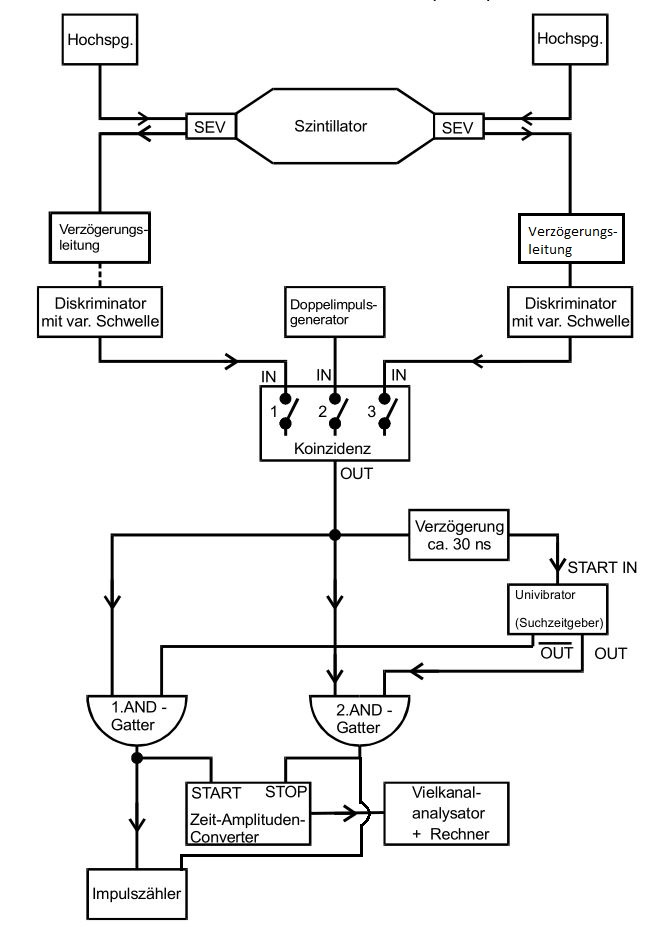
\includegraphics{blockschaltbild.JPG}
  \caption{Blockschaltbild der verwendeten Schaltung}
  \label{fig:schaltung}
\end{figure}
Also Szintillationsdetetektor wird ein Edelstahlzylinder mit aufgeschweisten Kegelstümpfen verwendet, der mit einem in Toluol gelösten, organischen Szintillator gefüllt
ist. Auf den Seitenflächen werden je ein an eine Hochspannung angeschlossener Sekundärelektronenvervielfacher (SEV) angeschlossen. Der SEV wird optisch an den Zylinder gekoppelt
und besteht aus einer Photokathode und Dynoden zur Signalverstärkung.\\
Weiterhin werden an beide SEV eine Verzögerungsschaltung und ein Diskriminator angeschlossen. Die Verzögerungsschaltung dienen dazu die Signale der SEV möglichst glechzeitig in
die Koinzidenzschaltung weiterzugeben. Der Diskriminator hat zwei für den weiteren verlauf nötige Funktionen.
\begin{itemize}
  \item[1.] Das durch z.B. thermische Elektronenemissionen in einem der SEV entstehende Untergrundrauschen wird durch einstellen einer Signalschwelle minimiert.
  \item[2.] Das einlaufende Signal wird in ein H/L-Signal der NIM-Logik übersetzt, damit die anschließend verwendeten Logikbausteine das Signal verarbeitn können.
\end{itemize}
Die aus den Diskriminatoren auslaufenden Signale werden nun auf eine Koinzidenzschaltung gegeben. Diese dient dazu diejenigen Signale auszusortieren, welche
durch durch Spontanemissionen in einem SEV entstehen. Wird ein Myon nah an einem der beiden SEV gemessen ist es möglich, dass die nachfolgende Schaltung die Messung
irrtümlich als fehlgeschlagen interpretiert, da die Lichtimpulse zu unterschiedlichen Zeiten von den SEV registriert werden. Dieses Problem wird ebenfalls durch die
Koinzidenzschaltung minimiert.\\
Aus der Koinzidenschaltung wird das Signal nun dreigeteilt und auf 2 AND-Gatter sowie durch eine weitere Verzögerung in eine monostabile Kippstufe geleitet.
Die Kippstufe wird ebenfalls an die beiden AND-Gatter angeschlossen. Wird nun ein Myon detektiert gibt zunächst das erste AND-Gatter ein H Signal weiter, bis nach $\SI{30}{\nano\second}$
die Stufe kippt und das H Signal am $\bar{\symup{OUT}}$ anliegt. Falls im Detektor nun ein zweiter Puls aufgenommen wird, wird dieser durch das zweite AND-Gatter als H Signal weitergeleitet.
Das erste Gatter registriert also den Eintritt und das zweite den Zerfall des Myons. Die Signale der Gatter werden nun von je einem Impulszähler registriert und in einen Zeit-Amplitude-Konverter (TAC)
geleitet. Dieser wandelt die zwischen den Pulsen vergehende Zeit in ein Signal mit Höhe proportional zur vergangen Zeit um. Diese Signale werden dann mithilfe eines Analog-Digital Konverters in einem 512-Bit
Vielkanalanalysator geleteitet. Die am TAC entstehenden Signale sind also repräsentativ für die Individuallebensdauern der Myonen.\\
\subsection{Kalibrierung und Messverfahren}
\label{sub:kalimes}
Bevor die eigentliche Messung durchgeführt werden kann wird die Schaltung der Reihe nach aufgebaut und das Signal mithilfe eines Oszilloskops visualisiert um die idealen Kenngrößen einzustellen.
Zu erst werden die Verzögerer richtig eingestellt und die länge der Spannungspulse wird vermessen.
Dann werden die Diskriminatoren angeschlossen und die Diskriminatorschwelle so eingestellt, dass beide Messkanäle ungefähr gleiche Zählraten liefern.
Auch hier wird die Länge der nun rechteckigen Pulse ausgelesen.\\
Als nächstes wird die Koinzidenzschaltung justiert. Dafür wird die Verzögerungszeit systematisch variiert und die unterschiedlichen Zählraten werden aufgenommen.
Das Maximum der entstehenden Kurve wird als ideale Verzögerungszeit eingestellt. Des weiteren wird die Zählrate vor und nach der Koinzidenzschaltung verglichen um sich von der Wirksamkeit der Schaltung
zu überzeugen.\\
Anschließed werden die Kippstufe, die AND-Gatter und der TAC angeschlossen. Am Ausgang des TAC kann nun die Suchzeit gemessen werden, in der die Stufe sich im gekippten Zustand befindet.
Die Suchzeit sollte dabei nur wenig größer sein als die Messzeit des TAC.
Mithilfe eines ebenfalls an die Koinzidenzschaltung angeschlossenen Doppelimpulsgenerators wird die Funktionsweise der Schaltung zur Registrierung des Stoppimpulses getestet.
Dies ist notwendig, da im späteren Experiment nur wenige der eintretenden Myonen auch im Detektor zerfallen. Am TAC wird nun außerdem überprüft ob die ausgehenden SIgnale proportional zum am Doppelimpulsgenerator
eingestellten Impulsabstand sind.\\
Zuletzt wird für den Vielkanalanalysator überprüft, welcher Kanal welcher Messzeit entspricht.\\
\\
Nun kann mit der eigentlichen Messung der Individuallebensdauern begonnen werden. Dafür werden Zählwerk und Vielkanalanalysator zeitgleich gestartet. Die Messung findet in einem Zeitraum von 20 bis 30h statt und
wird wiederum durch gleichzeitiges Stoppen der Zählwerks und des Vielkanalanalysators beendet. Die Ergebnisse des Vielkanalanalysators, sowie die Anzahl der detektierten Start- und Stoppimpulse werden aufgezeichnet
und die exakte Messzeit werden aufgezeichnet.\\
